
\section{Method}\label{sec:methods}
For this review, we followed the guidelines proposed by \cite{kitchenham2009systematic} and framed the search using the PICOC criteria \cite{petticrew2008systematic}:
\begin{itemize}
    \item \textbf{Population}: Applications, Developers
    \item \textbf{Intervention}: Collaborative, multi-user and interactive \gls{AR} applications
    \item \textbf{Comparison}: Students' results in classes using AR applications with classes that do not
    \item \textbf{Outcome}: Effectiveness in increasing understanding of a topic
    \item \textbf{Context}: Education, primary or secondary schools
\end{itemize}

Once the research questions have been defined, the literature review is split into three steps: planning, conducting and reporting. We used the online tool Parsifal\footnote{parsif.al} to conduct the first two steps of the review while the third was performed using Google Forms\footnote{https://forms.gle/D7NHktgfaRmAeWTS8} and collecting the results in a spreadsheet. The results of the data collection, as well as the code used to generate the figures in this document, are available on Github\footnote{github.com/Stocastico/AR\_SLR\_Paper}.


\subsection{Study selection}
The aim of this phase is to select the papers which are relevant for the systematic review, define the inclusion and exclusion criteria, and to provide the categories for the analysis.
We have selected publications from IEEExplore, Scopus, Springer and ISI Web of Science, as these four digital libraries collect a large amount of the research that is published in the area of technology enhanced learning. We used the search terms \emph{Augmented Reality}, \emph{Education} $\lor$ \emph{Learning}, \emph{Collaborative} $\lor$ \emph{Interactive} $\lor$ \emph{Multi-user}, \emph{Application} $\lor$ \emph{Evaluation}, as we wanted to include only papers that could help address RQ1 and RQ3. For this work, we only considered papers which appeared online from 2015 to the end of 2020. The search returned \allPapers results, of which \duplPapers were marked as duplicates. We read the abstract of the remaining \papersCheckAbstract articles and, applying the inclusion and exclusion criteria specified below, we were left with \papersToRead articles. We finally proceeded to read the selected articles and excluded \papersExludedAfterReading further articles, thus selecting \papersSelected articles for the literature review.
Table \ref{tab:searchstring} summarises the selection process, specifying the search string used for each digital library as well as the number of papers returned, marked as duplicated and selected for the systematic review.

As inclusion criteria, we required that the studies:
\begin{itemize}
    \item Were published from 2015 to 2020 (both inclusive);
    \item Describe an AR application  which has actually been implemented;
    \item Have a target audience of primary and/or secondary school students.
\end{itemize}

The decision of including only works with an audience comprised of primary or secondary students was taken because this study was conducted in the context of the ARETE H2020 European project\footnote{areteproject.eu}, studying multi-user AR applications for primary and secondary schools.

The exclusion criteria are the following:

\begin{itemize}
    \item The application described is not interactive, multi-user or collaborative;
    \item The paper does not describe an AR application
    \item The paper describes an unrelated application (e.g. for museums or clinical training);
    \item The paper is not peer reviewed;
    \item The paper is not written in English.
\end{itemize}

Fig. \ref{fig:flowchart} shows a flowchart depicting the systematic review process. The \papersToRead papers were reviewed, evenly split, by three researchers. To compute the interrater agreement, two researchers read a set of 50 abstracts randomly selected from all the studies (excluding duplicates) and 10 papers (among the \papersToRead eligible papers). The interrater agreement, as defined in \cite{cohen1960coefficient} was $0.88$ for the abstracts and $0.73$ for the papers.

\begin{figure}[htbp]	
	\begin{center}
	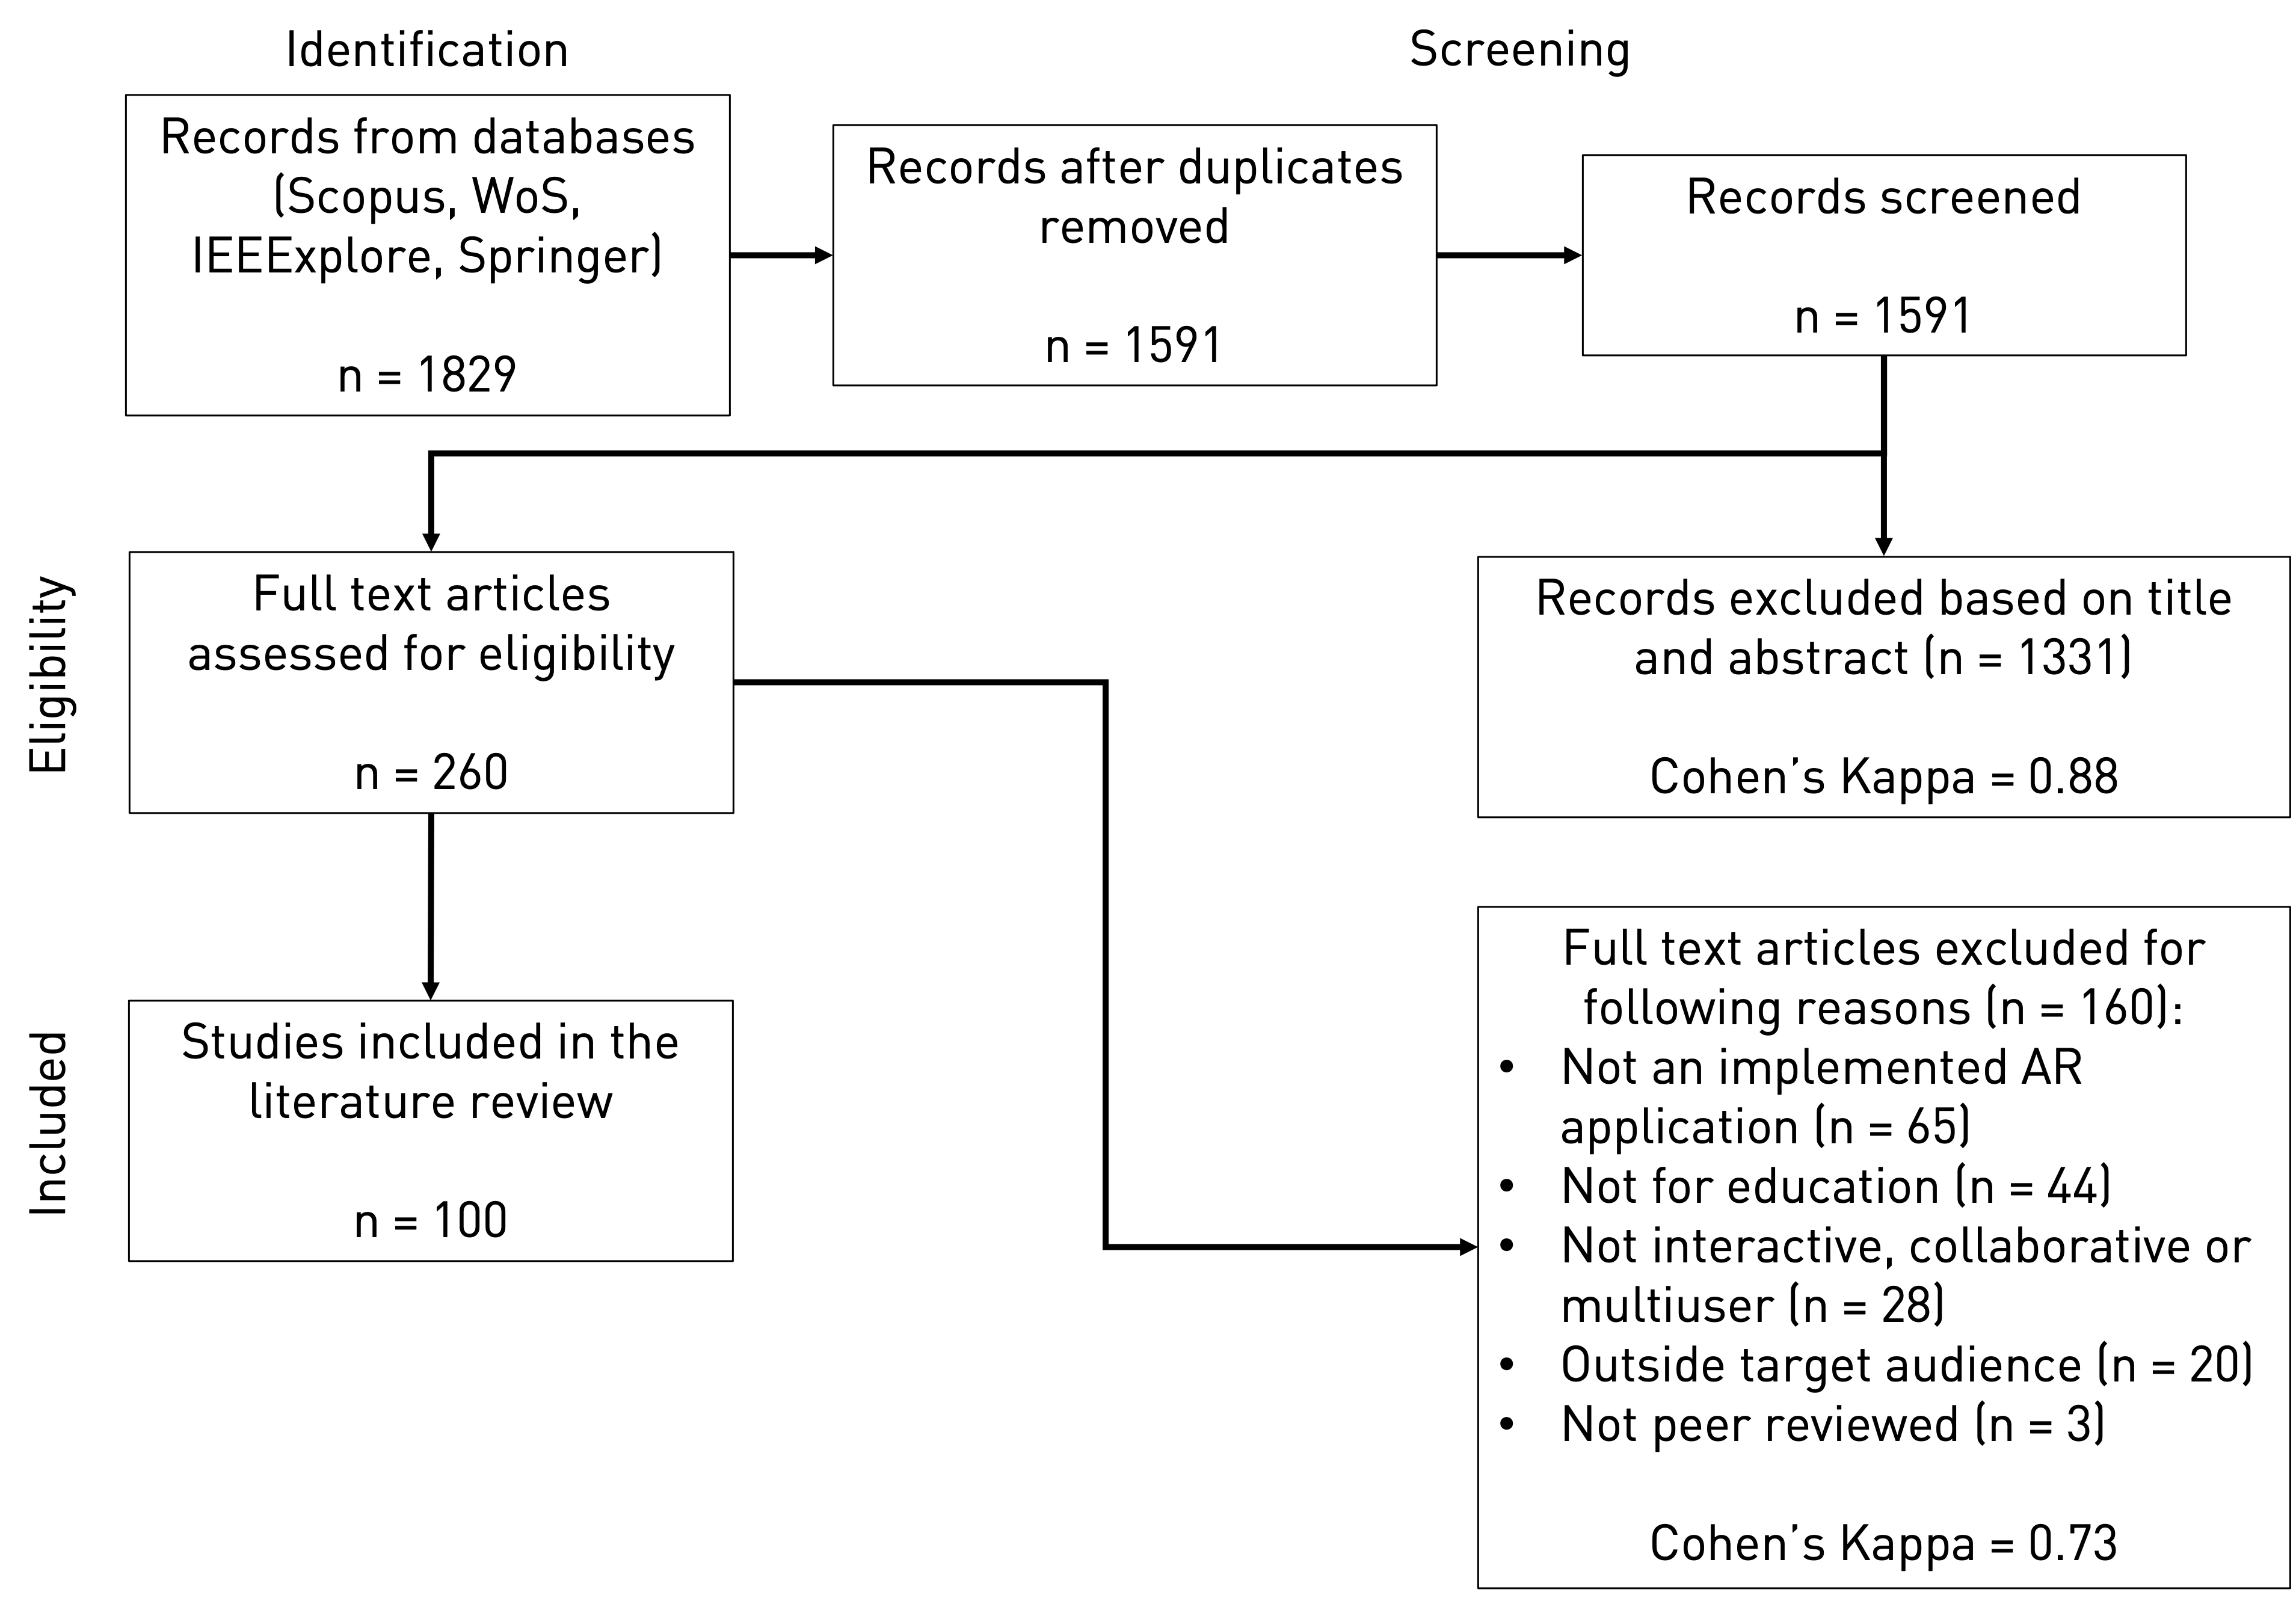
\includegraphics[width=0.8\textwidth]{figures/Prisma_flowchart_2.png}
	%\includegraphics[width=\textwidth]{figures/prisma_flowchart.png}
	\captionsetup{font=small}
	\caption{\fontsize{10pt}{11pt}\selectfont{\itshape{Prisma flowchart of the search protocol.}}}
	\label{fig:flowchart}
    \end{center}
\end{figure}


\begin{table*}[t]
\small
\begin{tabular}{M{1.9cm}M{6cm}M{1cm}M{1.65cm}M{1.15cm}}
    \toprule
         \textbf{Digital Library} & \textbf{Query string} & \textbf{Papers} & \textbf{Duplicates} & \textbf{Selected} \\
    \midrule
         IEEExplore    &  (``All Metadata'': ``Augmented reality'' AND (``Education'' OR ``Learning'') AND (``Collaborative'' OR ``Interactive'' OR ``multi-user'' OR ``multi-user'') AND (``Application'' OR ``Evaluation'')) Filters Applied: 2015 - 2020 & 136 & 48 & \textbf{37} \\
    \midrule
        Scopus         & TITLE-ABS-KEY ( ``Augmented reality''  AND  ( ``Education''  OR  ``Learning'' )  AND  ( ``Interactive''  OR  ``multi-user''  OR  ``multiuser'' OR ``collaborative'' )  AND  ( ``Application''  OR  ``Evaluation'' ) )  AND  ( PUBYEAR $>$ 2014 )  & 521 & 65 & \textbf{98} \\
    \midrule
        Springer       & (collaborative OR interactive OR multiuser OR multi-user) AND ``augmented reality'' AND (education OR learning) AND (primary OR secondary) AND (application OR evaluation)
        within Chapter - Conference Paper  2015 - 2020  & 904 & 69 & \textbf{72} \\
    \midrule
        Web of Science & ``Augmented reality'' AND (``Education'' OR ``Learning'') AND (``Collaborative'' OR ``Interactive'' OR ``multi-user'' OR ``multiuser'') AND (``Application'' OR ``Evaluation'') Filters Applied: 2015 - 2020 & 268 & 56 & \textbf{53} \\
    \bottomrule
\end{tabular}
\caption{\fontsize{10pt}{11pt}\selectfont{\itshape{Query strings and number of papers returned.}}}
\label{tab:searchstring}
\end{table*}